% !TeX root = ../main.tex
% Add the above to each chapter to make compiling the PDF easier in some editors.

\chapter{Implementations}\label{chapter:implementations}
This section explains the implementations and how to implement them efficiently.
As the shuffle operator-simulation is based on fixed-size tuples, the explanations of the following implementation, are based on fixed-size tuples as well.

\section{Partitioning}
We generate our tuples using an pseudo-random number generator.
To distribute the tuples into partitions, we use the following function:
\begin{equation}
  f(t) = t\textrm{.key}\ \%\ \textrm{partitions}
\end{equation}

As the modulo calculation is quite expensive, it we use the following partitioning function, when the count of partitions is a power of two:
\begin{equation}
  f(t) = t\textrm{.key}\ \&\ (\textrm{partitions - 1})
\end{equation}

\section{Slotted Pages}
Slotted pages store their information on fixed size memory blocks, that are split up in three sections: a fixed-size header, slots and a data section.
We are using slotted pages with a total size of 5 MiB per page.

\begin{figure}[h]
  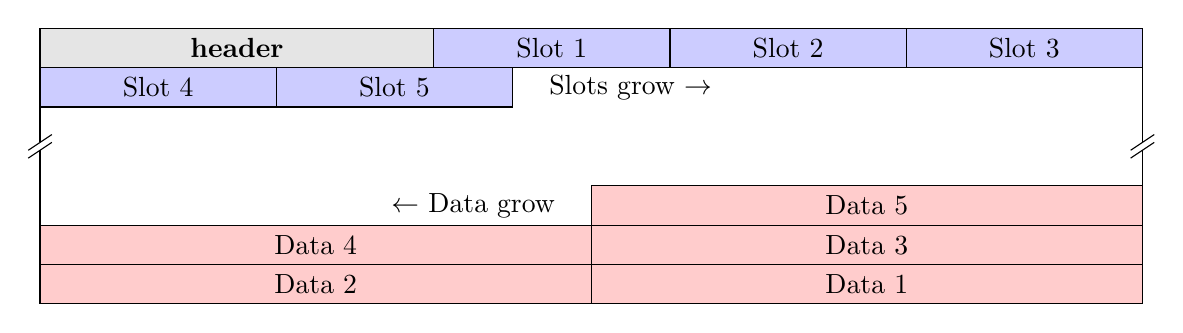
\begin{tikzpicture}
    % Page Outline
    \foreach \x in {0, 14}{
        \draw (\x,0) -- (\x,1.95);
        \draw (\x-0.15,1.85) -- (\x+0.15,2.05);
        \draw (\x,3) -- (\x,2.05);
        \draw (\x-0.15,1.95) -- (\x+0.15,2.15);
      }

    % Header Section
    \fill[gray!20] (0,3) rectangle (5,3.5);
    \node[anchor=center] at (2.5,3.25) {\textbf{header}};
    \draw (0,3) rectangle (5,3.5);

    % Slots Section
    \fill[blue!20] (5,3) rectangle (14,3.5);
    \fill[blue!20] (0,2.5) rectangle (6,3);

    % Slots (Fixed-size entries)
    \foreach \x in {5, 8, 11} {
        \draw (\x,3) rectangle (\x+3,3.5);
        \node[anchor=center] at (\x+1.5,3.25) {Slot \pgfmathparse{(\x-2)/3} \pgfmathprintnumber[precision=0]{\pgfmathresult}};
      }
    \foreach \x in {0, 3} {
        \draw (\x,2.5) rectangle (\x+3,3);
        \node[anchor=center] at (\x+1.5,2.75) {Slot \pgfmathparse{(\x)/3 + 4} \pgfmathprintnumber[precision=0]{\pgfmathresult}};
      }

    \node[anchor=center] at (6+1.5,2.75) {Slots grow $\rightarrow$};

    % Data Section
    \fill[red!20] (7,0) rectangle (14,1.5);
    \fill[red!20] (0,0) rectangle (14,1);

    \foreach \x in {14, 7} {
        \draw (\x,0) rectangle (\x-7,0.5);
        \node[anchor=center] at (\x-3.5,0.25) {Data \pgfmathparse{2-(\x)/7 + 1} \pgfmathprintnumber[precision=0]{\pgfmathresult}};
        \draw (\x,0.5) rectangle (\x-7,1);
        \node[anchor=center] at (\x-3.5,0.75) {Data \pgfmathparse{2-(\x)/7 + 3} \pgfmathprintnumber[precision=0]{\pgfmathresult}};
      }
    \draw (14,1) rectangle (7,1.5);
    \node[anchor=center] at (14-3.5,1.25) {Data \pgfmathparse{2-(14)/7 + 5} \pgfmathprintnumber[precision=0]{\pgfmathresult}};
    \node[anchor=center] at (7-1.5,1.25) {$\leftarrow$ Data grow};

  \end{tikzpicture}
  \centering
  \caption{Slotted Page grow visualization}
\end{figure}
In our implementation, we only store the tuple count in the header.
To construct our shuffle-simulation close to the real world usage, we split up each tuple.
In the slot information, we store the 4-Byte key together with data offset and length information.
The remainder of the tuple is then stored in the data section at the end of each page.

As we are using fixed-size tuples in our simulation, we only need to have the tuple slot index to be able to store the tuple on the page.
In constrast, when dealing with variable size tuples, slot index and data offset are needed to store a tuple.

\section{Slotted Page Managers}\label{section-slotted-page-managers}
As some implementation share the same tuple write-out strategy, we propose the used write-out strategies here and reference them in the following explanations of the concrete implementations.

To further simplify the implementations, we intialize each partition with an empty slotted page.
This significantly reduces the complexity of the page manager implementations.

\subsection{Lock-based Page Manager}
For each partition, we use a single lock and a vector for storing the slotted pages.
\begin{algorithm}[h]
  \caption{Lock-based Page Manager insert\_tuple Algorithm}\label{Lock-based-page-manager-insert-tuple}
  \SetKwInOut{Input}{input}\SetKwInOut{Output}{output}
  \Input{\texttt{tuple}: The tuple to be inserted, \texttt{partition}: The target partition index}
  \Output{Tuple inserted into the appropriate slotted page of the specified partition.}

  \SetKwFunction{Insert}{ insert\_tuple}

  \textbf{function}\Insert{tuple, partition}{

    Acquire lock on \texttt{partition\_locks[partition]}\; \eIf{pages[partition].back().add\_tuple(tuple)}{ // Tuple added successfully\; }{ add\_page(partition)\; pages[partition].back().add\_tuple(tuple)\; } Release lock\; } \end{algorithm} As can be seen in Algorithm \ref{Lock-based-page-manager-insert-tuple}, the lock-based insertion process is straightforward.
The insertion on a given slotted page, can only fail if the page is full.
This can easily be checked by reading the tuple count in the metadata section of the slotted page.
If the current page is full, we just allocate and append a new slotted page to the page vector of this partition.

\subsubsection*{Tuple insertion in batches}
Similarly, we can further optimize the write-out by using tuple-batches.
\begin{algorithm}[h]
  \caption{Lock-based Page Manager insert\_tuple\_batch Algorithm}\label{Lock-based-page-manager-insert-tuple-batch}
  \SetKwInOut{Input}{input}\SetKwInOut{Output}{output}
  \Input{\texttt{tuples}: The tuple-batch to be inserted\\ \texttt{partition}: The target partition index}
  \Output{Tuples inserted into one or more slotted pages of the specified partition.}

  \SetKwFunction{Insert}{ insert\_tuple\_batch}

  \textbf{function}\Insert{tuples, partition}{

    Acquire lock on \texttt{partition\_locks[partition]}\; \For{tuple : tuples}{ \eIf{pages[partition].back().add\_tuple(tuple)}{ // Tuple added successfully\; }{ add\_page(partition)\; pages[partition].back().add\_tuple(tuple)\; }} Release lock\; } \end{algorithm} In Algorithm \ref{Lock-based-page-manager-insert-tuple-batch}, we reuse the tuple insertion logic from Algorithm \ref{Lock-based-page-manager-insert-tuple} but acquire the partition lock only once for the entire insertion process.
Since acquiring and releasing the lock is expensive, this optimization significantly improves performance in multi-threaded scenarios.

\subsection{Lock-free Page Manager}
As holding a lock of a partition denies a second thread to also write out tuples, we propose a lock-free implementation.
In comparision to the lock-based variant, we now have to store our slotted pages in a pointer-stable data structure.
This is necessary to ensure threads can work simultanious, while a thread adds a new slotted page.
Furthermore, we have to edit the slotted page metadata using compare-and-exchange operations to avoid losing writes from other threads.

\begin{algorithm}[h]
  \caption{Lock-free Slotted Page increment\_and\_fetch\_opt\_write\_info Algorithm}\label{Lock-free-page-increment}
  \SetKwFunction{Increment}{ increment\_and\_fetch\_opt\_write\_info}
  \textbf{function}\Increment{}{

    current\_tuple\_count = header->tuple\_count.load();

    \While{!header->tuple\_count.compare\_exchange\_strong(current\_tuple\_count, current\_tuple\_count + 1)} {
      \If {current\_tuple\_count >= get\_max\_tuples(page\_size)} {
        return std::nullopt\;
      }
    }

    return \{page\_data.get(), page\_size, current\_tuple\_count\}\;
  }
\end{algorithm}
In order to gather the information, where we can write a tuple, we increment the tuple count using compare-and-exchange.
This index then acts as our location, where our tuple is placed on the page.
In Algorithm \ref{Lock-free-page-increment}, we also add an condition to stop attempting to further increase the count of tuples on the page, if the maximum is reached.
This ensures that threads move to the next allocated page.
Given the index, where the tuple is placed, we also append a pointer of the start of the page and the page size.
This ensures we can write the page without requiring any further information.

\begin{algorithm}[h]
  \SetKwFunction{Insert}{ insert\_tuple}
  \caption{Lock-free Page Manager insert\_tuple Algorithm}\label{Lock-free-page-manager-insert-tuple}
  \SetKwInOut{Input}{input}\SetKwInOut{Output}{output}
  \Input{\texttt{tuple}: The tuple to be inserted, \texttt{partition}: The target partition index}
  \Output{Tuple inserted into the appropriate slotted page of the specified partition.}
  \textbf{function}\Insert{tuple, partition}{

    wi = current\_page[partition].load()->increment\_and\_fetch\_opt\_write\_info()\;
    \While{wi == std::nullopt}{
      wi = current\_page[partition].load()->increment\_and\_fetch\_opt\_write\_info()\;
    }
    \If{wi.tuple\_index == LockFreeSlottedPage::get\_max\_tuples() - 1}{
      add\_page(partition)\;
    }
    LockFreeSlottedPage::add\_tuple\_using\_index(wi, tuple)\; } \end{algorithm} Using the Algorithm \ref{Lock-free-page-increment}, we retrieve the information to write the tuple in Algorithm \ref{Lock-free-page-manager-insert-tuple}.
We read from an atomically-stored pointer to our current page, until we are assigned an index on a slotted page.
If we are writing the last tuple on the page, we add a new page to this partition.
This is necessary to create a unqiue condition, when a new page has to be allocated.
With that write information at hand, we can write the tuple onto the slotted page.
\subsection{Histogram-based Page Managers}
The following page managers are based on histograms, which typically store tuple count and total tuple size per partition.
Similar to Section \ref{section:radix-partitioning}, this information can then be used to assign assign memory areas on slotted pages.
\subsubsection{Radix Page Manager} \label{subsubsection-Radix-Page-Manager}
This page manager applies the concept of radix-partitioning on slotted pages.
It uses an three step process:
\begin{enumerate}
  \item Histogram retrieval: Each thread reads its assigned materialized tuple chunk and builds up an histogram.
        As we are using fixed-size tuples, it only stores the tuple count per partition.
        This histogram is then forwared to the Radix Page Manager, which collects the histogram of each thread and then moves on to step 2.

  \item Page allocation: With all histograms at hand, the page manager sums up each histogram into a global histogram.
        This global histogram stores how many tuples each partition has to store.
        With that information we can allocate required pages for each partition.
        When all pages are ready to be used, step 3 begins.

  \item Assignment of slotted page sub-chunks: Each thread uses its local histogram to request storage locations for its tuples.
        The page manager uses the pre-allocated pages to assign each thread one or more memory chunks.
        These memory chunks can then be used exclusivly by the thread to store each tuples.
        Only the tuple count in the metadata has to be atomicly updated once, to signal that this thread has finished its work on this page.
        Otherwise, this write-out process does not rely on any synchronisation after the memory chunks.
\end{enumerate}
After these three steps are done, the page manager is finished.
Each page can be send to its receiver, once the expected tuple count is reached.
This can be done by the last thread to increment the tuple count.

\subsubsection{Ad-hoc Radix ("Hybrid") Page Manager} \label{subsubsection-Ad-hoc-Radix-Page-Manager}
The idea of the previous Radix Page Manager can be used to construct an approach, where each thread can hand in its histogram and receive memory chunks on slotted pages independently from other threads.
This page manager merges the three steps of the Radix Page Manager into one.

A thread hands in its histogram and request the memory chunks, where the tuples can be written.
The page manager reads the histogram and processes each partition individually.
For each partition, where a tuple has to be stored, the lock of the partition is aquired.
If there is any space left on a partition, it is used up and assigned to this thread.
When the current page is full, a new page is allocated and the page manager continues the assignment process.
These exclusive memory locations are then used by the thread to store its tuples.

In comparision to the Radix Page Manager, this page manager does not pre-allocate all necessary pages.
Instead it allocates the pages when needed.
Furthermore, a thread can already receive its memory chunks, while other threads are still constructing their histograms.
This allows this implementation to avoid materialization of all tuples.
\subsection{Thread-Local Pages and Merge-based Page Manager}
A further step into reducing the necessaty of synchronsation are thread-local slotted pages.
This slotted page management scheme can be split into two phases:
\begin{enumerate}
  \item Thread-local write-out: These slotted pages are exclusivly used by the owning thread and after the tuple processing is done, each thread hands in their pages.
        When the page manager has received all pages of each thread, the merging phase is started.

  \item Page merging: The page manager splits up all partitions onto the available threads.
        Each thread is then responsible for merging the slotted pages for each partition in the assigned partition range.
        To minimize tuple movement, the slotted pages a sorted decreasingly by the tuple count.
        Then the pages fewer tuples are merged into the fuller pages.
        It can be the cases that the last page cannot be fully merged into any other slotted page.
        Then this page has to be reordered so that the slots and data section start at the section beginnings.
        This is necessary to avoid having an gap at the beginnng of the slot or data section.
\end{enumerate}
After the merging phase, all tuples are stored on the least possible amount of slotted pages.
During the thread-local processing, it is likely that more slotted pages than necessary are created.
This can lead to an significant higher memory consumption than the previous approaches.
\subsection{Implementation-independent Optimizations}
We use the following optimizations to speed up our simulation of the shuffle operator.
\subsubsection{Padded atomics and locks}
All implementations, that use an array of partition locks, are affected by false sharing.
False sharing is caused when an cache line stores two independent values and one \ac{CPU} core is modifying the first value.
Then another CPU core wants to access the second value, which causes an cache miss.

This performance degration can be avoided by storing each individual partition lock aligned to the L1-cache line boundary.
This significantly reduces the amount of L1-cache misses, as the partition locks are frequently accessed.

\subsubsection{Minimal page-locking}
When holding a partition lock, the tuple write-out onto a slotted page is an expensive operation.
To reduce the lock-duration, we gather the necessary write-out information and prepare the next tuple insertion, and releasing the lock before the actual tuple write-out.

\subsubsection{Two-step buffered slotted page write out}
When writing out a batch of tuples onto a slotted page, we can process each tuple individually.
First, we construct the slot for the tuple, and then we store the variable-size data in the data section at the end of page.
Linux on an x86-64 machine, typically uses 4 KiB memory pages.
As we use 5 MiB slotted pages, it is expected that the slot and data are on different memory pages.

To reduce the amount simultanious accessed pages, we store our batches in a slot phase and a data phase.
As we are now writing to either the slot or data section, we switch between memory pages less often.
This is more friendly to the \ac{CPU} cache and the \ac{TLB}.

\section{On-Demand Partitioning} \label{section-On-Demand-Partitioning}
\subsection{Overview}
On-demand Partitioning is the simplest algorithm to implement the shuffle operator.
As soon as this implementation receives a batch of tuples, it processes each tuple individually.
First, the hash-function is applied onto the tuple to gather information in which partition this tuple belongs.
With this information, we can write out the tuple into the corresponding partition.

This implementation is compatible with the lock-based or lock-free Page Manager and the Thread-Local Pages and Merge-based Page Manager (see Section \ref{section-slotted-page-managers})

\subsection{Software Managed Buffers-based Partitioning}

This naive approach can be significantly improved by using \acfp{SMB}.
Instead of immediately writing out the tuple, it can be stored in a thread-locally allocated buffer.
The tuples, that belong do a partition, are stored in a dedicated area within this buffer.
As soon as this sub-region capacity is full, we write out the tuples to a slotted page.
Similarly, if all incoming tuples have been processed, we write out all remaining tuples inside the buffer.

This temporal storage brings another benefit.
We can now use the batch insertion features from the page managers.
Batch insertions are more \ac{CPU}-cache and \ac{TLB} friendly, as we switch our modified memory locations less often.

\section{Histogram-based Partitioning}
\subsection{Overview}
Similar to Radix Partitioning (see Section \ref{section:radix-partitioning}), a histogram can be used to assign threads memory location to store the tuples.
A histogram in the context of Radix Partitioning stores information like count of tuples and their total size per partition.
This information can then be used to assign each thread exactly the memory block it needs.

In our fixed-size tuple case, we only store the count of tuples of each partition.
As we have to construct the whole histogram, before the thread can store any tuples, we have to iterate over all tuples twice.
The first phase is necessary to create the histogram and receive memory locations to store the tuples.
The second phase then uses these memory locations to store the tuples.

Similar to On-Demand Partitioning (see Section \ref{section-On-Demand-Partitioning}), the proposed implementations below benefit from \acfp{SMB} to write out tuples in batches.
\subsection{Radix Partitioning}
This implementation naively implements Radix Partitioning on a stream of incoming tuple batches.
First, we fully materialize all generated tuples.
Then each thread receives a part of the materialized tuples.
Just like in the traditional Radix Partitioning, we construct the histogram for the assigned tuples.

The Radix Page Manager (see Section \ref{subsubsection-Radix-Page-Manager}) collects the histograms of all threads.
Each thread then receives their own, exclusive memory locations to store their tuples.
This allows us to store the tuples without any synchronisation.
Only the tuple count in the metadata section of each slotted page has to be updated atomically.
As soon as a slotted page reaches its proposed tuple count, it can be send to next downstream operator.

\subsection{Ad-hoc Radix ("Hybrid") Partitioning}
As the full materialization of all generated tuples and the wait times until the global histogram is created, are quite expensive, we propose a more efficent solution.
Instead of materializing all tuples, we process all incoming tuples morsel-driven.
For a given morsel, we then create an histogram.
The Ad-hoc Radix Page Manager (see Section \ref{subsubsection-Ad-hoc-Radix-Page-Manager}) uses this morsel-histogram to greedily assign this thread exclusive memory location to store the tuples.

Just like in the streaming Radix-Partitioning case above, the tuples are stored on each slotted page without needing synchronisation.
The tuple count in the metadata section also requires synchronsiation in form of an atomic tuple count.
As the morsel size are smaller than the assigned part of the materialized tuples, this counter has to be increased more often.
%\section{Thread-Local Pages and Merge-based Partitioning}
%\subsection{Overview}

\section{Collaborative Morsel Processing}
\subsection{Overview}
In the previous implementations, each thread can write out to each partition.
We avoid invalid writes by using locks or atomic operation.
Shared usage of locks or atomics causes contention and frequent cache invalidations.

To reduce contention, we assigning each thread a partition range.
A thread will only write out a tuple, if the partitioning function maps it to a partition within this partitioning range.
Nevertheless, we still have to partition all tuples to their correct partition.
Because of that, we have to process each tuple in a way that it can be stored any partition.
Thus, a tuple must be processed by a group of threads, where the union of their individual partition ranges covers all possible partitions.
\subsection{Collaborative Morsel Processing with exclusive partition ranges}
This implementation constructs the partition ranges so that it fufills two conditions:
\begin{enumerate}
  \item Any partition range does not overlap with any other partition range.
  \item The union of all partition ranges results in a complete coverage of all possible partitions.
\end{enumerate}
With these two conditions in place, we avoid having to syncronize the tuple write-out process.
But we have to process each tuple $p$ times, where $p$ is the number of partition ranges.
As the incoming tuples only have to be read, they typically can reside in the L2 or L3 \ac{CPU} caches.

Assuming uniform distribution across all partitions, the implementations efficiency decreases with increasing CPU core count.
If we distribute the partitions into fair partition ranges, the likelyhood of a given tuple to be partitioned in a given partition range is:
\begin{equation}\label{equation-CMP-exclusive-partition-ranges}
  \Pr[X=\textrm{Partition Range}_i] \approx \frac{1}{p},  \quad \forall i
\end{equation}
As we want to increase the amount of partition ranges ($p$) with increasing core count, the likelyhood that a thread processes a tuple for its assigned partition range decreases.
\subsection{Collaborative Morsel Processing using processing units}
As we can see in the above \ac{CMP} with exclusive partition ranges implementation, exclusive partition ranges theoretical performance does not scale well.
This implementation aims to reduce this impact by using processing units.
A processing unit is a partition of $t$ threads, that split up the total partitions into $t$ fair, exclusive partition ranges.
Again, within a processing unit, no partition ranges overlap.

When we use multiple processing units, we have to synchronise the tuple write-out again.
In constrast to previous implementations without exclusive partition ranges, each partition can be written by only one thread per processing unit.
This significantly reduces the contention on the synchronisation mechanism of each partition.

Furthermore, each tuples has to be only processed by a single processing unit.
Assuming we fairly split up our $c$ \ac{CPU} cores into $pu$ processing units, then each processing unit will have around $t\approx\frac{c}{pu}$ threads to process tuples.
When we increase to count of CPU cores and processing units in a similar manner, then the amount of threads per processing unit remains constant.
This means our likelyhood of processing a tuple, that belongs to into the partition range of a randomly-selected thread is:
\begin{equation}\label{equation-CMP-PU}
  \Pr[X=\textrm{Partition Range}_i] \approx \frac{1}{t},  \quad \forall i
\end{equation}

When we compare the approximation in \ref{equation-CMP-exclusive-partition-ranges} and \ref{equation-CMP-PU}, it is visible that as long as we keep the ratio between CPU cores and processing units constant, the processing efficieny remains constant.
In contrast, when using \acl{CMP} with exclusive partition ranges the amount of exclusive partition ranges increases with the CPU core count.
This then leads to a decrease of processing efficiency when increasing the CPU cores.
\section{Complexity Analysis}
\subsection{Time Complexity}
$\Theta(n)$

Proof Idea: Lower bound trivial, upper bound bank method
\subsubsection{Tuple Access Count}
\subsection{Space Complexity}
$\Theta(n)$

Proof Idea: Lower bound trivial, upper bound bank method
\subsubsection{Memory Consumption}
